\documentclass[crop,tikz]{standalone}

\usepackage{tikz}
\usepackage{anyfontsize}

\usetikzlibrary{bending}
\usetikzlibrary{arrows.meta}
\begin{document}


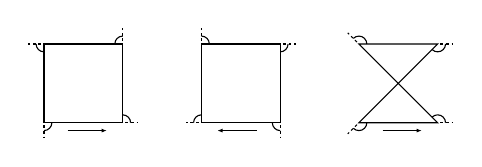
\begin{tikzpicture}[dash1/.style={dashed,dash pattern=on 1pt off 1pt, dash phase=1pt}]

\draw (0,0) -- (1,0) -- (1,1) -- (0,1) -- cycle;
\draw[dash1] (0,0) -- (0,-0.2);
\draw[dash1] (1,0) -- (1.2,0);
\draw[dash1] (1,1) -- (1,1.2);
\draw[dash1] (0,1) -- (-0.2,1);

\draw ([shift=(270:0.1)]0,0) arc [radius=0.1, start angle=-90, end angle= 0  ];
\draw ([shift=(0  :0.1)]1,0) arc [radius=0.1, start angle=0  , end angle= 90 ];
\draw ([shift=(90 :0.1)]1,1) arc [radius=0.1, start angle=90 , end angle= 180];
\draw ([shift=(180:0.1)]0,1) arc [radius=0.1, start angle=180, end angle= 270];

\draw [arrows = {-Latex[scale=0.4]}] (0.3, -0.1) -- (0.8, -0.1);

\draw (2,0) -- (3,0) -- (3,1) -- (2,1) -- cycle;
\draw[dash1] (2,0) -- (1.8,0);
\draw[dash1] (3,0) -- (3,-0.2);
\draw[dash1] (3,1) -- (3.2,1);
\draw[dash1] (2,1) -- (2,1.2);

\draw [arrows = {-Latex[scale=0.4]}] (2.7, -0.1) -- (2.2, -0.1);

\draw ([shift=(180:0.1)]2,0) arc [radius=0.1, start angle=180, end angle= 90 ];
\draw ([shift=(90 :0.1)]2,1) arc [radius=0.1, start angle=90 , end angle= 0 ];
\draw ([shift=(0 :0.1)]3,1) arc [radius=0.1, start angle=0 , end angle= -90];
\draw ([shift=(-90:0.1)]3,0) arc [radius=0.1, start angle=-90, end angle=-180];

\draw [arrows = {-Latex[scale=0.4]}] (4.3, -0.1) -- (4.8, -0.1);

\draw (4,0) -- (5,0) -- (4,1) -- (5,1) -- cycle;
\draw[dash1] (4,0) -- ([shift=(225:0.2)]4,0);
\draw[dash1] (5,0) -- (5.2,0);
\draw[dash1] (4,1) -- ([shift=(135:0.2)]4,1);
\draw[dash1] (5,1) -- (5.2,1);

\draw ([shift=(-135:0.1)]4,0) arc [radius=0.1, start angle=-135, end angle= 0 ];
\draw ([shift=(0 :0.1)]5,0) arc [radius=0.1, start angle=0 , end angle= 135 ];
\draw ([shift=(135  :0.1)]4,1) arc [radius=0.1, start angle=135 , end angle= 0];
\draw ([shift=(0:0.1)]5,1) arc [radius=0.1, start angle=0, end angle= -135];

\end{tikzpicture}

\end{document}